\chapter{Results}\label{ch:results}

In this chapter we will try to answer our subquestions using the results we obtained\footnote{https://tensorboard.dev/experiment/1YZvra2iQseNTMWDeBFREw/} after training and testing our models.

\iffalse
\textsl{What is the effect on the performance and efficiency of using linear transformers in an inpainting context for anomaly detection when compared to regular transformers?}

To be able to compare the different models we ask a few subquestions:
\begin{itemize}
    % inpainting/anomaly detection/localisation
    \item Do we see a difference in detection of anomalies across images with different textures and objects?
    \item Do we see a difference in segmentation of anomalies across images with difference textures and objects?
    % performance/efficiency
    \item How does the training time compare across images with different textures and objects?
    \item How does the training time compare between the full and linear attention models?
    % linear vs regular
    \item How do our results compare to previous work?
\end{itemize}
\fi

\section{Detection \& Segmentation}
\label{sec:results:det-seg}

\textsl{What is the difference between softmax and linear attention in detection of anomalies across images with different textures and objects?}

The AUROC \% scores of our MSA and MLSA models are given by table \ref{table:results:segdet}. The best models for each image have been indicated by bold text.

This shows that for detection the MLSA-based models outperform the MSA-based models the majority of the textured images. The wood and leather categories are the exceptions. The difference between the MSA and MLSA models is particularly high in the carpet, grid and leather categories.

The results for detection on the object images are split equally over MSA and MLSA. The values for the cable and pill categories are very low, especially when compared to the other images. 

\

\textsl{What is the difference between softmax and linear attention in segmentation of anomalies across images with difference textures and objects?}

The results for segmentation across the textured images is very similar when compared to the numbers for detection. MSA seems to perform worse for three out of the five textured images. The same is true for the object images. The differences for the capsule, hazelnut and metal nut between MSA and MLSA are especially high. MLSA has a higher score for all these cases with at least a difference of 7\%. Interestingly MSA seems to perform better on average when the image size is larger.

\

Let us analyse results for some specific cases with low and high model performance. Looking at the figure \ref{fig:results:leather-anomap} we see that the mask and the segmentations of the anomaly for the leather category do not match, only the center of the anomaly is correctly localised. This explains the low AUROC value. Looking at the reconstructions in figure \ref{fig:results:leather-recon} we see that both the models using MSA and MLSA are missing details, which means that the average training error used to calculate the anomaly map affects the results. For the better performing grid category we see in figure \ref{fig:results:grid-anomap} that the anomalies are correctly localised, with the MSA model having more noise in the anomaly map around the sides.

\begin{figure}[ht!]
\centering
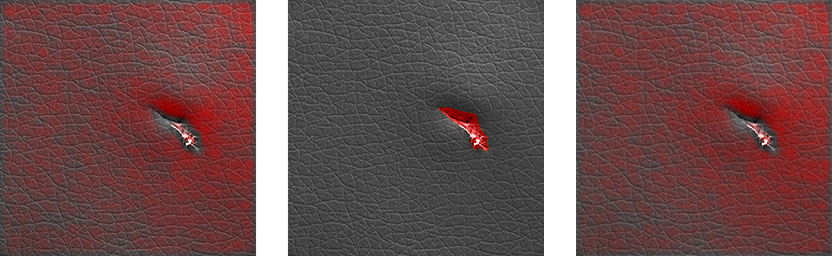
\includegraphics[width=\textwidth]{imgs/samples/leather_cut_anomap.jpg}
\caption{Example of an anomalous image from the leather category comparing MSA, the dataset mask and MLSA}
\label{fig:results:leather-anomap}
\end{figure}

\begin{figure}[ht!]
\centering
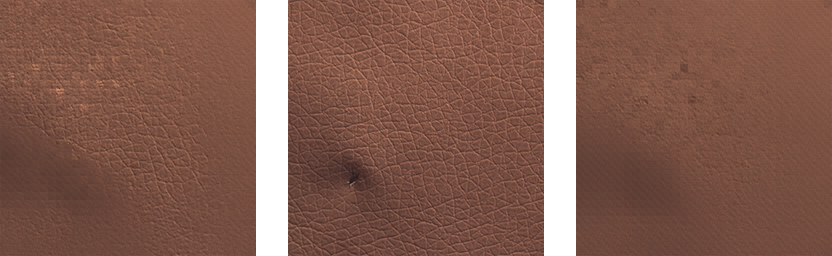
\includegraphics[width=\textwidth]{imgs/samples/leather_poke_recon.jpg}
\caption{Example of reconstructions from the leather category comparing MSA, the original and MLSA}
\label{fig:results:leather-recon}
\end{figure}

\begin{figure}[ht!]
\centering
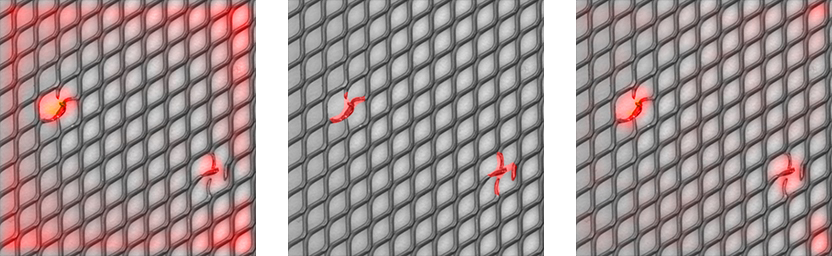
\includegraphics[width=\textwidth]{imgs/samples/grid_broken_anomap.jpg}
\caption{Example of an anomalous image from the grid category comparing MSA, the dataset mask and MLSA}
\label{fig:results:grid-anomap}
\end{figure}

It is interesting to see that the models do not perform the best for the majority of the images for both detection and segmentation, but only for one of these tasks. Since the score for detection depends on the anomaly map that is used to calculate the score for segmentation we would expect the segmentation score to directly relate to the detection score. However, the detection score is only a maximum pixel value which means it only represents one pixel of the anomaly map not taking into account the other values of the anomaly map. The segmentation score does look at all pixels.



\

Overall our results show that MLSA has better performance than MSA, both for segmentation and detection on textured and object images. And for detection on texture images.

\iffalse
\begin{itemize}
\item Detection on textured is MLSA best, only the carpet and grid seem to actually really do much better
\item Segmentation on textured is MSA best, which is interesting since detection uses those same values. Which could mean that there are a lot of false-positives for the detection -> needs a graph example
\item Wood seems to do the best in all cases, need to check the images to see what is different with the other textures

\item Segmentation on objects: MLSA is best, detection we see 50/50
\item Especially for detection there are a few very low values: cable & pill
\item Image size of pill & screw is 320 & 512 which is the largest and is also where MSA wins
\item On average MLSA does seem to perform better, so depending on how much time it takes it to train it could be a good alternative
\end{itemize}
\fi

\begin{table}
\centering
\resizebox{\linewidth}{!}{%
\begin{tabular}{l|cc|cc|c} 
\toprule
Category        & \multicolumn{2}{l}{MSA}  & \multicolumn{2}{l}{MLSA} & Image size  \\ 
\midrule
                & Segmentation & Detection & Segmentation & Detection &             \\ 
\midrule
Carpet          & 90.44        & 77.09     & \textbf{91.52}        & \textbf{86.40}     & 512         \\
Grid            & 89.82        & 76.61     & \textbf{93.39}        & \textbf{89.97}     & 256         \\
Leather         &  49.99       & \textbf{86.85}     &     \textbf{56.23}    & 75.44     & 512         \\
Tile            & \textbf{79.31}        & 71.32     & 73.33        & \textbf{73.92}     & 512         \\
Wood            & \textbf{70.22}        & \textbf{77.54}     & 62.84        & 72.72     & 512         \\ 
\midrule
Texture average & \textbf{75.96} &	77.88 &	75.46 &	\textbf{79.69} &             \\ 
\midrule
Bottle          & 65.82        & \textbf{91.51}     & \textbf{68.65}        & 89.92     & 256         \\
Cable           & 88.04        & 38.17     & \textbf{90.07}        & \textbf{43.65}     & 256         \\
Capsule         & 81.66        & \textbf{72.32}     & \textbf{88.43}        & 66.33     & 320         \\
Hazelnut        & 67.94        & \textbf{55.89}     & \textbf{81.59}        & 53.82     & 256         \\
Metal nut       & 54.99        & 60.95     & \textbf{67.51}        & \textbf{78.49}     & 256         \\
Pill            & \textbf{88.60}        & 44.82     & 88.45        & \textbf{51.28}     & 320         \\
Screw           & \textbf{97.31}        & 55.69     & 97.23        & \textbf{65.32}     & 320         \\
Toothbrush      & 80.42        & 86.67     & \textbf{81.78}        & \textbf{87.22}     & 256         \\
Transistor      & 77.72        & \textbf{59.25}     & \textbf{79.95}        & 56.71     & 256         \\
Zipper          & \textbf{81.22}        & \textbf{79.07}     & 79.66        & 78.07     & 512         \\ 
\midrule
Object average  & 78.37        & 64.43     & \textbf{82.33}        & \textbf{67.08}     &             \\ 
\midrule
All average     & 80.02        & 66.46     & \textbf{81.32}        & \textbf{70.00}     &             \\
\bottomrule
\end{tabular}
}
\label{table:results:segdet}
\caption{Results in AUROC \% for segmentation and detection}
\end{table}




\section{Efficiency}
\label{sec:results:efficiency}

\textsl{How does the number of epochs required to get the best result compare across images with different textures and objects?}\

The number of epochs required depends on the type of image. Image that have more complex structures require more epochs. We see this especially in the texture category and for the cable, screw and transistor images. Another factor affecting the number of epochs is the amount of colours used. This is shown by the pill and zipper images that both require a very low number of epochs and primarily consist of black, white and grey colours. We give some samples of the image categories in figure \ref{fig:results:detail-samples}.

\begin{figure}[ht!]
\centering
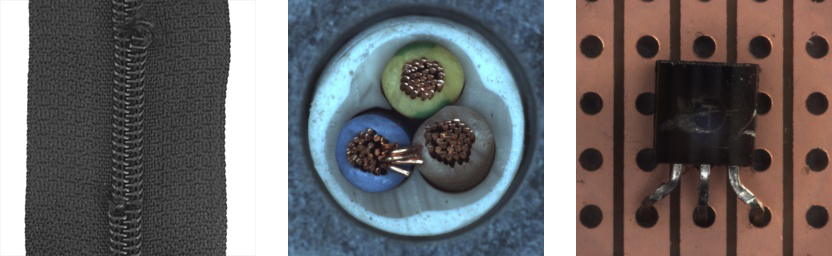
\includegraphics[width=\textwidth]{imgs/samples/image-detail-sample.jpg}
\caption{Examples of the zipper, cable and transistor image types}
\label{fig:results:detail-samples}
\end{figure}

\textsl{How does the training time compare between the softmax and linear attention models across images with different textures and objects?}\

We see that the time per epoch is lower for MSA in all categories except for the pill and transistor images. With this information we would expect the MSA models to also finish training faster. The opposite is true however. The number of epochs required for the best result is lower in eleven of the fifteen cases, which also means that the total training time is lower for MLSA.

\iffalse
\begin{itemize}
    \item Time per epoch is lower for MSA in all categories except for pill and transistor
    \item Less epochs to get the best result in the case of MSA: 2, 11 for MLSA, 3 the same
    \item The above would mean that given the number of epochs is lower, the total time is also lower
    \item given that in the previous section it is also better in the task the linear model is slightly better
    \item Training time does highly depend on the category, but there is no clear difference except for the object images with a solid background seem to require less training time.
    \item The pill and zipper images that are technically black/white do require the lowest number of epochs
\end{itemize}
\fi

\begin{table}
\centering
\resizebox{\linewidth}{!}{%
\begin{tabular}{l|ccc|ccc} 
\toprule
Category   & \multicolumn{3}{l}{MSA}                 & \multicolumn{3}{l}{MLSA}                 \\ 
\midrule
~          & Best epoch & Time/Epoch & Training time & Best epoch & Time/Epoch & Training time  \\ 
\midrule
Carpet     & \textbf{77}         & \textbf{0:58:05}    & \textbf{220:42:00}     & 138        & 1:07:17    & 265:47:00      \\
Grid       & 140        & \textbf{0:26:48}    & 130:00:00     & \textbf{53}         & 0:33:34    & \textbf{114:06:00}      \\
Leather    & 142        & 0:43:50    & 214:03:00     & 142        & \textbf{0:43:33}    & \textbf{213:24:00}      \\
Tile       & \textbf{353}        & 0:36:40    & \textbf{308:01:00}     & 555        & \textbf{0:39:38}    & 466:23:00      \\
Wood       & 149        & 0:53:56    & 270:33:00     & \textbf{124}        & \textbf{0:56:16}    & \textbf{258:49:00}      \\
\midrule
Bottle     & 37         & \textbf{0:24:11}    & 75:47:00      & \textbf{11}         & 0:24:33    & \textbf{66:16:00}       \\
Cable      & 250        & \textbf{0:39:59}    & 267:55:00     & \textbf{211}        & 0:48:07    & \textbf{267:05:00}      \\
Capsule    & 27         & \textbf{0:41:38}    & 123:30:00     & \textbf{14}         & 0:41:45    & \textbf{114:50:00}      \\
Hazelnut   & 83         & \textbf{1:22:12}    & 321:56:00     & \textbf{19}         & 1:25:10    & \textbf{242:43:00}      \\
Metal nut  & 148        & \textbf{0:25:31}    & 127:10:00     & \textbf{43}         & 0:28:22    & \textbf{91:42:00}       \\
Pill       & 5          & 0:48:57    & 128:06:00     & \textbf{4}          & \textbf{0:46:54}    & \textbf{121:57:00}      \\
Screw      & 245        & \textbf{0:40:27}    & 267:01:00     & \textbf{211}        & 0:40:37    & \textbf{245:04:00}      \\
Toothbrush & 58         & 0:12:19    & 42:55:00      & 58         & \textbf{0:12:10}    & \textbf{42:24:00}       \\
Transistor & 271        & 0:46:40    & 328:13:00     & \textbf{196}        & \textbf{0:44:59}    & \textbf{260:57:00}      \\
Zipper     & 5          & \textbf{0:25:59}    & \textbf{67:34:00}      & 5          & 0:34:52    & 90:39:00       \\
\bottomrule
\end{tabular}
}
\label{table:results:times}
\caption{Best epochs and time taken to finish training}
\end{table}

\section{Comparison with previous work}

\textsl{How do our results compare to previous work?}

When we compare our results those from the original InTra model by Pirnay et al. \cite{pirnay_inpainting_2021} in table \ref{table:results:pirnay} we see that the performance of our models is worse than the original model. The only result that is better is the segmentation for the carpet image type. This was to be expected, since we have omitted some parts of the original InTra model that improved their results. We will discuss those choices in chapter \ref{ch:discussion}.

\begin{table}
\centering
\begin{tabular}{l|cc} 
\toprule
Category        & \multicolumn{2}{l}{InTra}    \\ 
\midrule
                & Segmentation & Detection    \\ 
\midrule
Carpet          & 88.2         & 98           \\
Grid            & 98.8         & 100          \\
Leather         & 99.5         & 100          \\
Tile            & 94.4         & 98           \\
Wood            & 88.7         & 97          \\ 
\midrule
Texture average & 96.1         & 98           \\ 
\midrule
Bottle          & 97.1         & 100          \\
Cable           & 91.0         & 70           \\
Capsule         & 97.7         & 86           \\
Hazelnut        & 98.3         & 95         \\
Metal nut       & 93.3         & 96          \\
Pill            & 98.3         & 90          \\
Screw           & 99.5         & 95          \\
Toothbrush      & 98.9         & 100         \\
Transistor      & 96.1         & 95          \\
Zipper          & 99.2         & 99          \\ 
\midrule
Object average  & 96.9         & 93          \\ 
\midrule
All average     & 96.6         & 95          \\
\bottomrule
\end{tabular}
\label{table:results:pirnay}
\caption{Results from \cite{pirnay_inpainting_2021}}
\end{table}

\iffalse
\begin{itemize}
    \item Results are much worse
    \item Different attention function
    \item No connections between layers
    \item No augmentations
\end{itemize}
\fi